\documentclass[11pt]{scrartcl}
\usepackage{ebb}



\title {Problemas Diarios}
\subtitle {Ponte a entrenar ps}

\author{Emmanuel Buenrostro}

\begin{document}
\maketitle
\tableofcontents



Si entrenan IMC intenten los problemas de IMC, si no ¿pa que? (estos no vienen necesariamente en orden). \\

De OMM vienen 2 problemas, el 2do suele estar algo más dificil (o eso intento). \\

Los problemas que pongo usualmente no conozco la sol, pero si no les sale vemos como sale y si hay algo de teoria util pues lo vemos. \\

Creo que lo ideal es que si estan en IMC intenten los 2 de IMC y el 1 de OMM, y si estan en OMM intenten los 2 de OMM. \\

Aunque no se presionen hacer 2 problemas de OMM al dia es bastante y a veces los dias estan más saturados de lo normal (o lo normal es que esten muy saturados), y a veces los problemas estan muy dificiles, igual cualquier cosa pregunten este es todo el punto. \\

Asumo que el plan podria hacer eventualmente checar soluciones, podriamos hacerlo por texto o hacerlo por llamada (aunque creo que estan muy saturados de llamadas, y yo de cetichamba).

Las fuentes de los problemas se los pongo como 2 dias despues o asi 

\newpage
\section{Febrero}
\subsection{16 de Febrero}
\textbf{IMC: }
\indicacion{Creo que lo ideal es que lo intenten como IMC (tratar de sacarlo lo más rapido posible, los que digan que solo respuesta pueden asumir cosas que no demuestran pero confian en que son verdad (aunque despues si pruebenlo bien pues))}
\begin{problem} [IMC 2001/13]
    Sean $a,b$ dos reales positivos diferentes, sea $A=\frac{a+b}{2}$ y $G=\sqrt{ab}$. Prueba la siguiente desigualdad:
    \[G < \frac{(a-b)^2}{8(A-G)}<A\]
\end{problem}

\begin{problem}  [IMC 2005/10]
    Sea $a=9 \left[ n\left( \frac{10}{9}\right)^n-1-\left( \frac{10}{9}\right)-\left( \frac{10}{9}\right)^2-\ldots-\left( \frac{10}{9}\right)^{n-1}\right]$, donde $n$ es un entero positivo. Si $a$ es un entero, determina el maximo valor de $a$.
\end{problem}

\textbf{OMM:}

\problemdiff{4}
\problemtags{Combi, Invarianza, Coloraciones}
\begin{problem} [OMM 2017/1]
    
    En un tablero de ajedrez de $2017 \times 2017$, se han colocado en la primera columna $2017$
caballos de ajedrez, uno en cada casilla de la columna. Una tirada consiste en elegir dos
caballos distintos y de manera simulátnea moverlos como se mueven los caballos de ajedrez.
Encuentra todos los posibles valores enteros de $k$ con $1 \leq k \leq 2017$, para los cuales es
posible llegar a través de varias tiradas, a que todos los caballos están en la columna $k$, uno
en cada casilla.
Nota. Un caballo se mueve de una casilla $X$ a otra $Y$, solamente si $X$ y $Y$ son las esquinas
opuestas de un rectángulo de $3 \times 2$ o de $2 \times 3$.
    
\end{problem}

\begin{problem} [IMOSL 2019 C2]
    Se te da un conjunto de $n$ bloques, cada uno con peso al menos $1$; su peso total es $2n$. Demuestra que para todo número real $r$ con $0 \leq r \leq 2n - 2$, puedes elegir un subconjunto de los bloques cuyo peso total sea al menos $r$ pero a lo más $r + 2$.
\end{problem}
\begin{remark*}
    Lo traduci con GPT porque me dio flojera, aqui esta en ingles por si GPT tradujo mal:
    \begin{problem*}
    You are given a set of $n$ blocks, each weighing at least $1$; their total weight is $2n$. Prove that for every real number $r$ with $0 \leq r \leq 2n-2$ you can choose a subset of the blocks whose total weight is at least $r$ but at most $r + 2$.
    \end{problem*}
\end{remark*}


\newpage
\subsection{17 de Febrero}
\textbf{IMC:}
\begin{problem} [IMC 2018/2]
    Sean $m,n$ enteros positivos tales que $m(n-m)=-11n+8$. Encuentra la suma de todos los posibles valores de $m-n$.
\end{problem}

\begin{problem} [IMC 2006/8]
    El cuadrado $ABCD$ tiene lado $2$. $E$ y $F$ son los puntos medios de $AB,AD$ respectivamente. $G$ es un punto en $CF$ tal que $3CG=2GF$. Determina el area de $BEG$.
\end{problem}

\textbf{OMM:}
\begin{problem} [OMCC 1999/1]
    
    Se supone que $5$ personas conocen, cada una, informaciones parciales diferentes sobre cierto asunto. Cada vez que la persona $A$ llama a la persona $B$, $A$ le da a $B$ toda la información que conoce en ese momento sobre el asunto, mientras que $B$ no le dice nada de él. ¿Cuál es el mínimo número de llamadas necesarias para que todos lo sepan todo sobre el asunto? ¿Cuántas llamadas son necesarias si son $n$ personas?
\end{problem}

\begin{problem} [APMO 2023/2]
    Find all integers $n$ satisfying $n \geq 2$ and $\dfrac{\sigma(n)}{p(n)-1} = n$, in which $\sigma(n)$ denotes the sum of all positive divisors of $n$, and $p(n)$ denotes the largest prime divisor of $n$.
\end{problem}

\newpage
\subsection{18 de Febrero }

\textbf{IMC:}
\begin{problem} %[IMC 2016/9]
    Tres lineas paralelas $L_1, L_2$ y $L_3$ son tales que $L_1$ esta 1 cm arriba de $L_2$ y $L_3$ esta dos centimetros abajo de $L_2$. Un triangulo isosceles recto tiene uno de sus vertices en cada linea. ¿Cuál es la suma, en $\text{cm}^2$, de todos los posibles valores para el área de este triangulo?.
\end{problem}

\begin{problem} %[IMC 2014/6]
    Si $x,y,z$ son tres enteros positivos consecutivos tales que $\frac xy+\frac yz+\frac zx +\frac yx+\frac xz+\frac zy$ es un entero. ¿Cuál es el valor de $x+y+z$?.
\end{problem}

\textbf{OMM:}
\begin{problem} %[OMCC 2009/5]
    
    Dado un triángulo agudo y escaleno $ ABC$, sea $ H$ su ortocentro, $ O$ su circuncentro, $ E$ y $ F$ los pies de las altitudes trazadas desde $ B$ y $ C$, respectivamente. La recta $ AO$ vuelve a cortar la circunferencia del triángulo en el punto $ G$ y los segmentos $ FE$ y $ BC$ en los puntos $ X$ e $ Y$ respectivamente. Sea $ Z$ el punto de intersección de la recta $ AH$ y la recta tangente a la circunferencia en $ G$. Demostrar que $ HX$ es paralela a $ YZ$.
\end{problem}

\begin{problem} %[IMO SL 2009/G2]
    	Let $ABCD$ be a cyclic quadrilateral whose diagonals $AC$ and $BD$ meet at $E$. The extensions of the sides $AD$ and $BC$ beyond $A$ and $B$ meet at $F$. Let $G$ be the point such that $ECGD$ is a parallelogram, and let $H$ be the image of $E$ under reflection in $AD$. Prove that $D,H,F,G$ are concyclic.
\end{problem}

\newpage 

\subsection{19 de Febrero}
\textbf{IMC: }
\begin{problem} %[IMC 2006/4]
    El profe dijo, "Yo tengo dos números $a$ y $b$ que cumplen $a+b-ab=1$. Si te digo que $a$ no es un entero, ¿Qué puedes afirmar sobre $b$?". Alex dijo "Entonces $b$ tampoco es un entero". Brian dijo, "No, Yo pienso que $b$ debe ser algun entero positivo". Colin dijo,"No yo creo que $b$ debe ser algun entero negativo". ¿Quién tiene la razon? 
\end{problem}

\begin{problem} %[IMC 2006/2]
    El segmento $AB$ tiene longitud 5. En un plano que contiene a $AB$, ¿cuantas rectas estan a distancia $2$ de $A$ y $3$ de $B$?
\end{problem}

\textbf{OMM:}
\begin{problem} %[ORO 2016/6]
    The vertices of a regular polygon with $2016$ sides are colored gold or silver. Prove that there are at least $512$ different isosceles triangles whose vertices have the same color.
\end{problem}

\begin{problem} %[IMO SL 2010/G1]
    Let $ABC$ be an acute triangle with $D, E, F$ the feet of the altitudes lying on $BC, CA, AB$ respectively. One of the intersection points of the line $EF$ and the circumcircle is $P.$ The lines $BP$ and $DF$ meet at point $Q.$ Prove that $AP = AQ.$
\end{problem}

\newpage
\subsection{20 de Febrero}
\textbf{IMC:}
\begin{problem} %[IMC 2024/8]
    En la imagen hay 14 puntos en un circulo. ¿De cuántas formas se puede dibujar 7 cuerdas que no se intersequen? (Dos cuerdas no pueden tener extremos en común).
    \begin{center}
        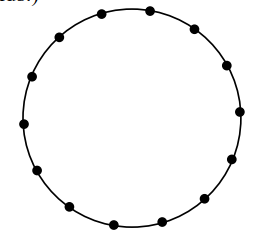
\includegraphics{24IMC8.png}
    \end{center}
\end{problem}

\begin{problem} %[IMC 2014/11]
    Considera todos los enteros positivos menores a 10000000000 en los cuales todos los digitos son 0 o 2. ¿Cuál es el total de 0s entre todos sus digitos?. 
\end{problem}

\textbf{OMM:}
\begin{problem} %[OMCC 2008/1]
    
    Encontrar el menor número entero positivo $ N$ tal que la suma de sus dígitos sea 100 y la suma de los dígitos de $ 2N$ sea 110.
\end{problem}

\begin{problem} %[OMCC 2016/6]
    
    Sea $\triangle ABC$ un triángulo con incentro $I$ y circuncírculo $\Gamma$. Sean $M=BI\cap \Gamma$ y $N=CI\cap \Gamma$, la recta paralela a $MN$ por $I$ corta a $AB$, $AC$ en $P$ y $Q$. Demostrar que el circunradio de $\odot (BNP)$ y $\odot (CMQ)$ son iguales.
\end{problem}

\newpage
\subsection{23 de Febrero}
\textbf{IMC:}

\begin{problem} %[IMC 2002/3]
    Para encontrar el valor de $x^8$ dado $x$ necesitas 3 operaciones aritmeticas: $x^2=x \cdot x$, $x^4=x^2\cdot x^2$, y $x^8=x^4\cdot x^4$. Para encontrar $x^{15}$ ocupas cinco operaciones: las primeras 3 son las mismas que en el anterior, luego $x^{16}=x^8 \cdot x^8$ y $x^{15}=x^{16}\div x$. ¿Cuál es el minimo de operaciones aritmeticas que ocupas para encontrar el valor de $x^{1000}$.
\end{problem}

\begin{problem} %[IMC 2006/9]
    Determina el valor de $x+y$ donde $x, y$ son números reales que cumplen 
    \[(2x+1)^2+y^2+(y-2x)^2 =\frac 13\]
\end{problem}

\textbf{OMM:}
\begin{problem} %[OMCC 2014/5]
    Points $A$, $B$, $C$ and $D$ are chosen on a line in that order, with $AB$ and $CD$ greater than $BC$. Equilateral triangles $APB$, $BCQ$ and $CDR$ are constructed so that $P$, $Q$ and $R$ are on the same side with respect to $AD$. If $\angle PQR=120^\circ$, show that

\[\frac{1}{AB}+\frac{1}{CD}=\frac{1}{BC}.\]
\end{problem}

\begin{problem} %[OMCC 2018/6]
    
    En La Habana se realiza un baile con $2018$ parejas. Para el baile, se dispone de una circunferencia donde inicialmente se marcan $2018$ puntos distintos, etiquetados con los números $0,1,\ldots,2017$. Las parejas son ubicadas sobre los puntos marcados, una en cada punto. Para $i\ge1$, se define $s_i$ como el residuo de dividir $i$ entre $2018$ y $r_i$ como el residuo de dividir $2i$ entre $2018$. El baile comienza en el minuto $0$. En el $i-$ésimo minuto después de haber inciado el baile, la pareja ubicada en el punto $s_i$ (si la hay) se mueve al punto $r_i$, la pareja que ocupaba el punto $r_i$ (si la hay) se retira, y el baile continúa con las parejas restantes. El baile termina después de $2018^2$ minutos. Determine cuantas parejas quedarán al terminar el baile.

    
\end{problem}

\newpage
\subsection{24 de Febrero }

\textbf{IMC:}
\begin{problem} %[IMC 2013/11]
    Los enteros positivos $a<b$ son tales que $\frac{a+b}{2}$ y $\sqrt{ab}$ son enteros positivos que consisten de los mismos dos digitos en orden inverso. ¿Cuál es el minimo valor posible de $a$? 
\end{problem}

\begin{problem} %[IMC 2007/3]
    En un triangulo $ABC$, $E$ es un punto en $AC$ y $F$ es un punto en $AB$. $BE$ y $CF$ se intersecan en $D$. Si las áreas de los triangulos $BDF,BCD$ y $CDE$ son $3,7$ y 7 respectivamente, ¿Cuál es el área de el cuadrilatero $AEDF$?
\end{problem}

\textbf{OMM:}
\begin{problem} %[OMM 2012/4]
    
    A cada entero positivo se le aplica el siguiente proceso: al número se le resta la suma de sus dígitos, y el resultado se divide entre $9$. Por ejemplo, el proceso aplicado al $938$ es $102$, ya que  $\frac{938-(9+3+8)}{9}=102$. Aplicado dos veces el proceso a $938$ se llega a $11$, aplicado tres veces se llega a $1$, y aplicado cuatro veces se llega al $0$. Cuando a un entero positivo $n$ se le aplica el proceso una o varias veces, se termina en $0$. Al número al que se llega antes de llegar al cero, lo llamamos la casa de $n$. ¿ Cuántos
números menores que $26000$ tienen la misma casa que el $2012$?
    
\end{problem}

\begin{problem} %[MEX TST 2024/5/2]
    Sean $x,y,z$ números reales positivos tales que $x+y+z=1$. Muestra que
    \[\sum_{\text{cyc}}\frac{x^2-yz}{x^2+x} \leq 0\]
\end{problem}
\end{document}